%label:"fig:lagrangianCobordism"
%author:JeffHicks
%name:"Lagragian cobordism"
%type:"figure"
%parent:"def:lagrangianCobordism"
%caption:"The projection of a Lagrangian cobordism $K\subset X\times \CC$ to the $\CC$ factor. This cobordism has ends  $K:(L_0, L_1, \ldots L_k)\rightsquigarrow \emptyset.$"




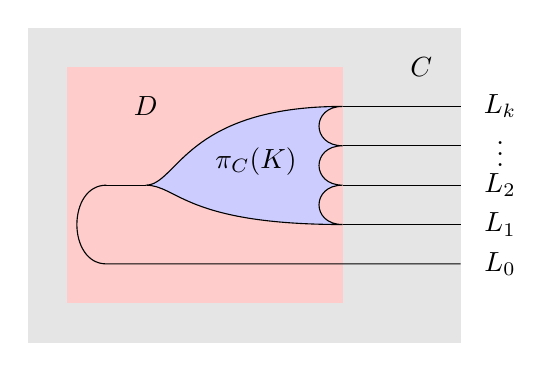
\begin{tikzpicture}[xscale=-1]
    \fill[fill=gray!20]  (-2,-2.5) rectangle (3.5,1.5);
    \fill[red!20]  (-0.5,-2) rectangle (3,1);
        \draw[fill=blue!20] (-0.5,-1) .. controls (-0.1,-1) and (-0.1,-0.5) .. (-0.5,-0.5) .. controls (-0.1,-0.5) and (-0.1,0) .. (-0.5,0) .. controls (-0.1,0) and (-0.1,0.5) .. (-0.5,0.5) .. controls (1.5,0.5) and (1.6,-0.5) .. (2,-0.5) .. controls (1.6,-0.5) and (1.5,-1) .. (-0.5,-1);
        \draw (-2,-1) -- (-0.5,-1);
        \draw (-2,-0.5) -- (-0.5,-0.5);
        \draw (-2,0) -- (-0.5,0);
        \draw (-2,0.5) -- (-0.5,0.5);
        \draw (2,-0.5) -- (2.5,-0.5);
        \node at (-2.5,0.5) {$L_k$};
        \node at (-2.5,0) {$\vdots$};
        \node at (-2.5,-0.5) {$L_2$};
        \node at (-2.5,-1) {$L_1$};
        \node at (-2.5,-1.5) {$L_0$};
        \node at (0.6,-0.2) {$\pi_{\mathbb C}(K)$};
    \draw (2.5,-0.5) .. controls (3,-0.5) and (3,-1.5) .. (2.5,-1.5) .. controls (2,-1.5) and (-1.5,-1.5) .. (-2,-1.5);
    
    \node at (2,0.5) {$D$};
    \node at (-1.5,1) {$\mathbb C$};
    \end{tikzpicture}